
The game works as intended with the operations being correctly evaluated
 and the gameboard updating correctly to reflect all the changes. The score updates correctly on deletion of full rows, with greater weights 
being given to deleting more rows simultaneously. The game correctly ends on any coloumn being filled. \\
A quick gameplay run showing this can be seen in the video linked at:

\begin{align}
    \centering
    \textnormal{\url{https://shorturl.at/etvQ9}} \nonumber
\end{align}

\begin{figure}[ht]
    \centering
    \begin{subfigure}[b]{0.4\textwidth}
        \centering
        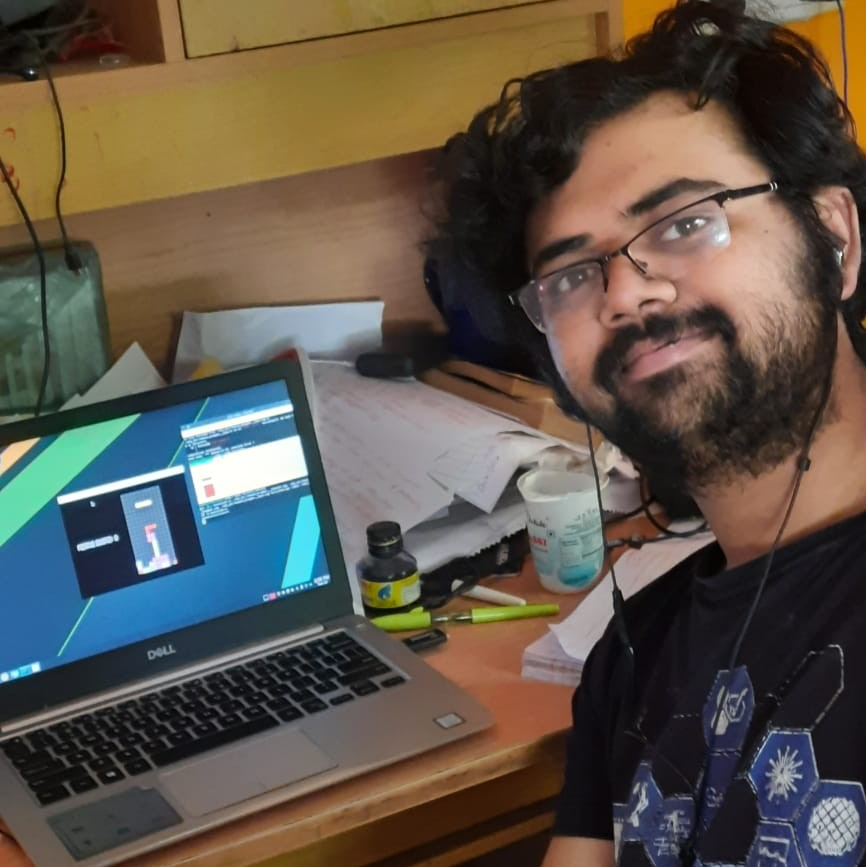
\includegraphics[width=\textwidth]{fig/demo-pushk.jpeg}
    \end{subfigure}
%
    \begin{subfigure}[b]{0.4\textwidth}
        \centering
        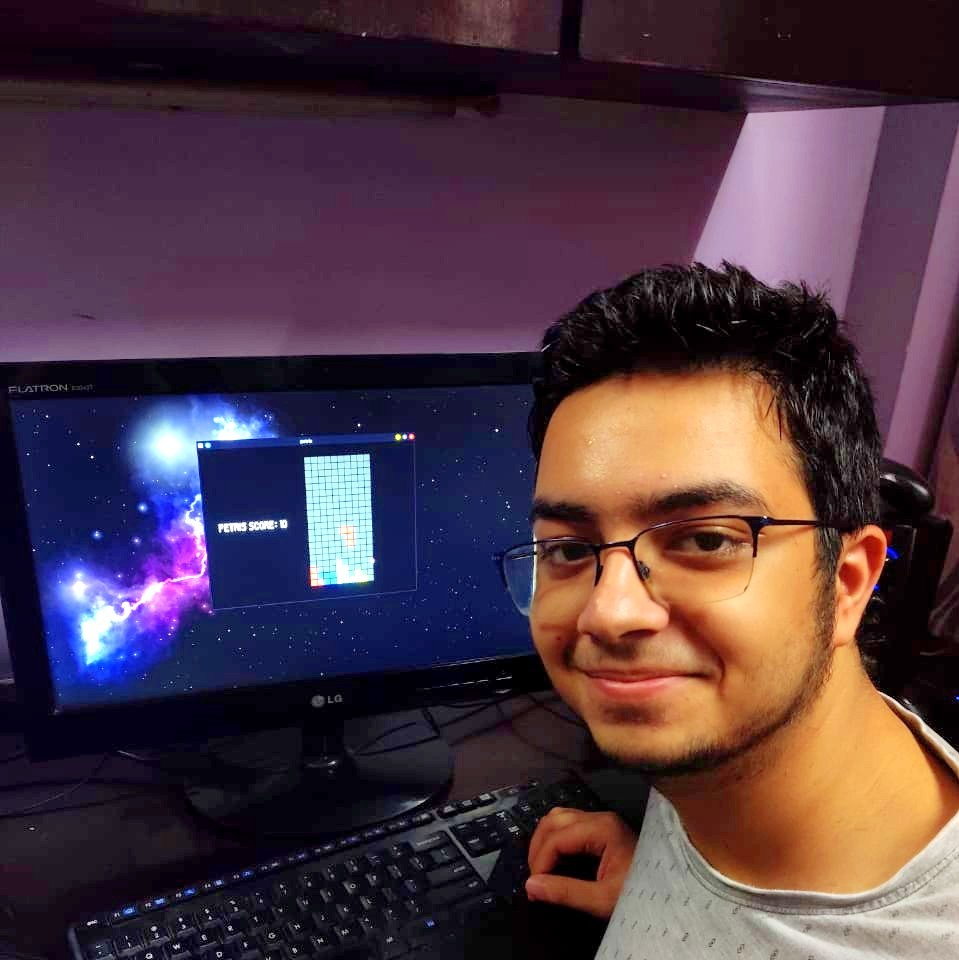
\includegraphics[width=\textwidth]{fig/demo-sank.jpeg}
    \end{subfigure}
    \caption{\emph{Look Ma! No FPGA!}}
\label{fig:demo}
\end{figure}


There are several optimizaions and additional features that can be implemented. Implementations to the User Interface could include
\begin{itemize}
    \item A game reset button that allows you to play multiple games on one execution
    \item A high score display that keeps track of your best performances
\end{itemize}
Potential optimizations to the game would include
\begin{itemize}
    \item Improving the framerate of the VGA simulator
    \item Introducing more parallel updating for the game logic, which it is currently not due to synchronization and framerate issues. This currently doesn't matter 
     due to the low framerate being the rate determining step but this should definitely be done if using a real FPGA 
\end{itemize}

The project can be found at our GitHub repository: \url{https://github.com/sankalpgambhir/petris}.

